\documentclass[11pt]{article}
\usepackage[margin=1in]{geometry}
\usepackage{booktabs,longtable,array,graphicx,enumitem}
\usepackage[hidelinks]{hyperref}
\setlength{\parindent}{0pt}
\setlength{\parskip}{6pt}
\renewcommand{\arraystretch}{1.15}
\newcommand{\plainbox}[1]{\par\vspace{2pt}\noindent\fbox{\parbox{\dimexpr\linewidth-2\fboxsep-2\fboxrule\relax}{#1}}\par\vspace{2pt}}
\begin{document}
{\Large\textbf{Tasks Module, Part 3: General Results}}\par
{\large What the task answers show about all 13 jobs, before we look at any ropeway job}\par\vspace{4pt}\hrule\vspace{8pt}

\plainbox{\textbf{Remember.} These results come from \textbf{made-up} answers for 104 imaginary workers (see Part 2).
They show that the methods work and what the output looks like. They are not findings about real workers.}

\section*{1. What we did, in one paragraph}
For each worker we have 27 answers: does this task \emph{regularly} in the main job (answer 1), \emph{did it before} elsewhere (answer 2), or never.
We first use only answer 1 (called the \textbf{strict} view: what the person does now). Then we add answer 2 (the \textbf{broad} view: what the person has done at some time).
We start with the whole picture, and leave the ropeway jobs to Part 4.

\section*{2. How many tasks does a worker do?}
The average worker does \textbf{7.4} of the 27 tasks regularly. The range is 2 to 16.
The average worker has also done \textbf{1.9} more tasks before, elsewhere, so about 9.4 in the broad view.
79 in 100 workers report at least one task done before.
\begin{center}
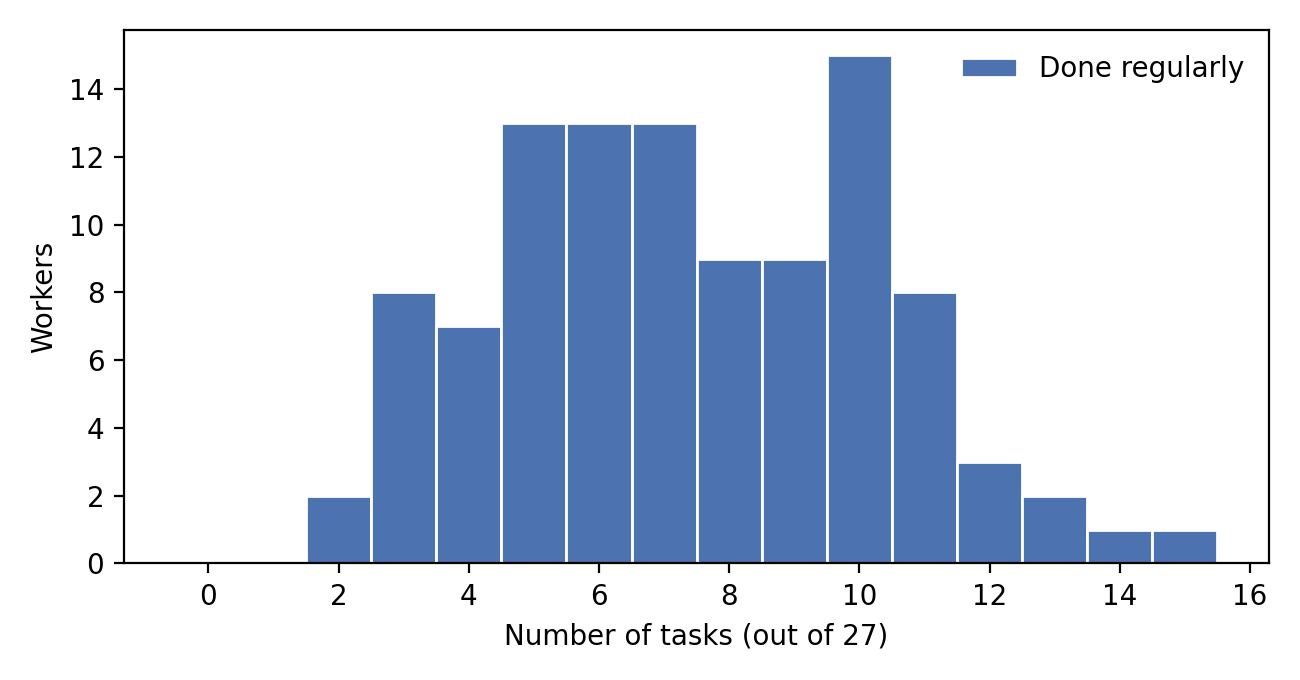
\includegraphics[width=0.7\linewidth]{../03_analysis/outputs/3_1_hist.png}\\[2pt]
{\small Number of tasks done regularly, by worker.}
\end{center}

{\small
\begin{longtable}{lrrrrr}
\toprule
\textbf{Job} & \textbf{Workers} & \textbf{Regular (avg)} & \textbf{Range} & \textbf{Before (avg)} & \textbf{Both (avg)} \\
\midrule
\endfirsthead
\toprule
\textbf{Job} & \textbf{Workers} & \textbf{Regular (avg)} & \textbf{Range} & \textbf{Before (avg)} & \textbf{Both (avg)} \\
\midrule
\endhead
Pony business & 5 & 10.6 & 7--16 & 1.4 & 12.0 \\
Hotel/lodging owner & 7 & 10.0 & 6--14 & 2.0 & 12.0 \\
Shop owner & 11 & 8.4 & 4--11 & 1.7 & 10.1 \\
Dhaba/food-stall owner & 6 & 8.3 & 3--13 & 1.3 & 9.7 \\
Driver & 7 & 8.1 & 3--13 & 2.7 & 10.9 \\
Shopkeeper & 14 & 7.4 & 4--10 & 2.1 & 9.6 \\
Pony worker & 5 & 7.4 & 5--10 & 0.4 & 7.8 \\
Palki & 6 & 7.2 & 3--11 & 0.7 & 7.8 \\
Porter & 10 & 6.9 & 2--12 & 1.2 & 8.1 \\
Hotel/lodging worker & 15 & 6.8 & 4--12 & 2.7 & 9.5 \\
Guide & 3 & 5.7 & 2--8 & 1.7 & 7.3 \\
Wage labourer & 11 & 5.6 & 3--8 & 3.1 & 8.7 \\
Other & 4 & 4.2 & 3--7 & 1.5 & 5.8 \\
\bottomrule
\end{longtable}
}

Owners do more tasks than workers: they sell, handle money, buy stock and supervise. Wage labourers report the most work done before, as we built them to (they often work in other trades in the off-season).
\textbf{Small groups.} Guides (3 workers) and ``Other'' (4 workers) are too few to say anything on their own. In the real survey they need a top-up sample or must be pooled.

\section*{3. Which jobs do which tasks?}
The picture below has one row per job and one column per task. Dark means most workers in that job do the task regularly.
Each job has a clear ``signature'': porters and wage labourers carry loads (1) and load and unload (3);
owners sell (14), bargain (15), handle cash (16) and supervise (26); drivers drive (7) and check the vehicle (9); the palki job carries a passenger (2).
\begin{center}
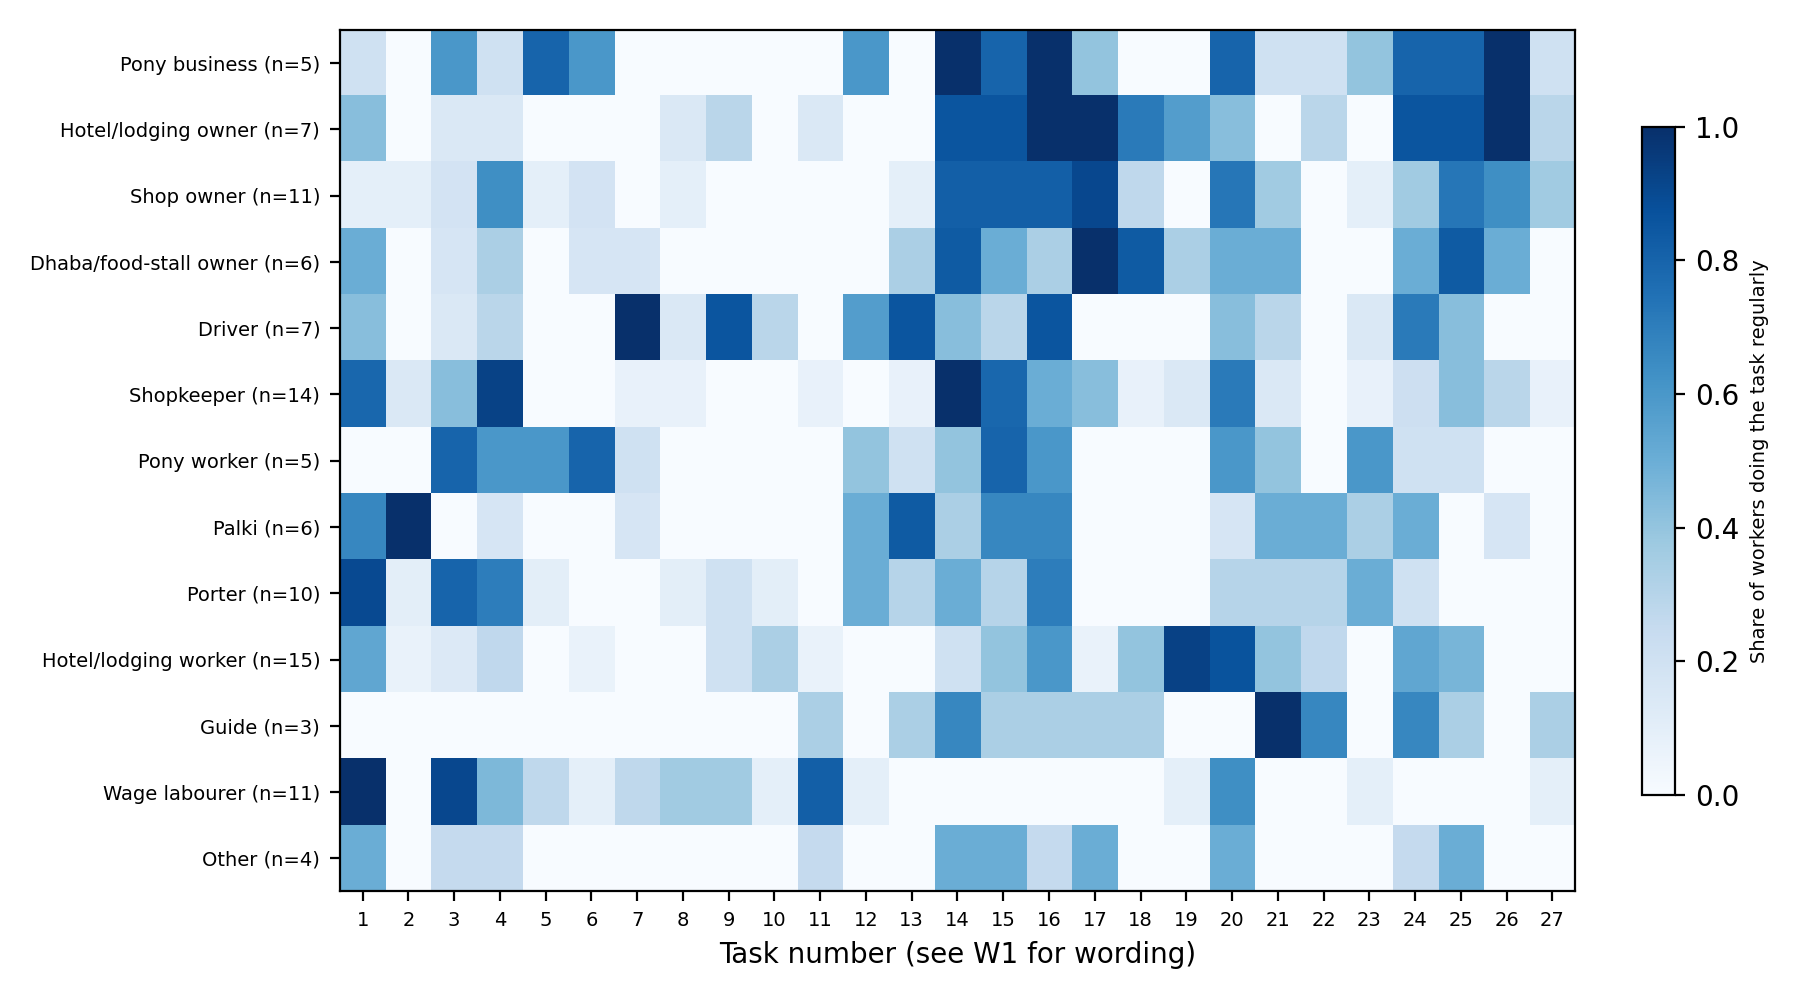
\includegraphics[width=1.0\linewidth]{../03_analysis/outputs/3_2_heatmap.png}\\[2pt]
{\small Share of workers in each job who do each task regularly. Task numbers are listed in Part 1.}
\end{center}

\textbf{Most common tasks} across all workers: handle cash and payments (59\%); clean rooms or public areas (58\%); sell goods or services (56\%).
\textbf{Least common}: operate an engine or machine (9\%); electrical or wiring work (9\%); teach or train others (10\%).
A task that few people do is not useless for our purpose. Electrical work or running an engine can be exactly what a ropeway job needs, so the count of people who do it matters most when we compare against jobs in Part 4.

\section*{4. Broad task groups}
We sorted the 27 tasks into three broad groups: \emph{hands-on} (16 tasks), \emph{dealing with people} (7) and \emph{thinking and counting} (4).
Overall, workers spend 51 in 100 of their regular tasks on hands-on work,
32 on dealing with people and 18 on thinking and counting.
These shares depend partly on how many tasks fall in each group, so compare jobs with each other rather than with 100.
\begin{center}
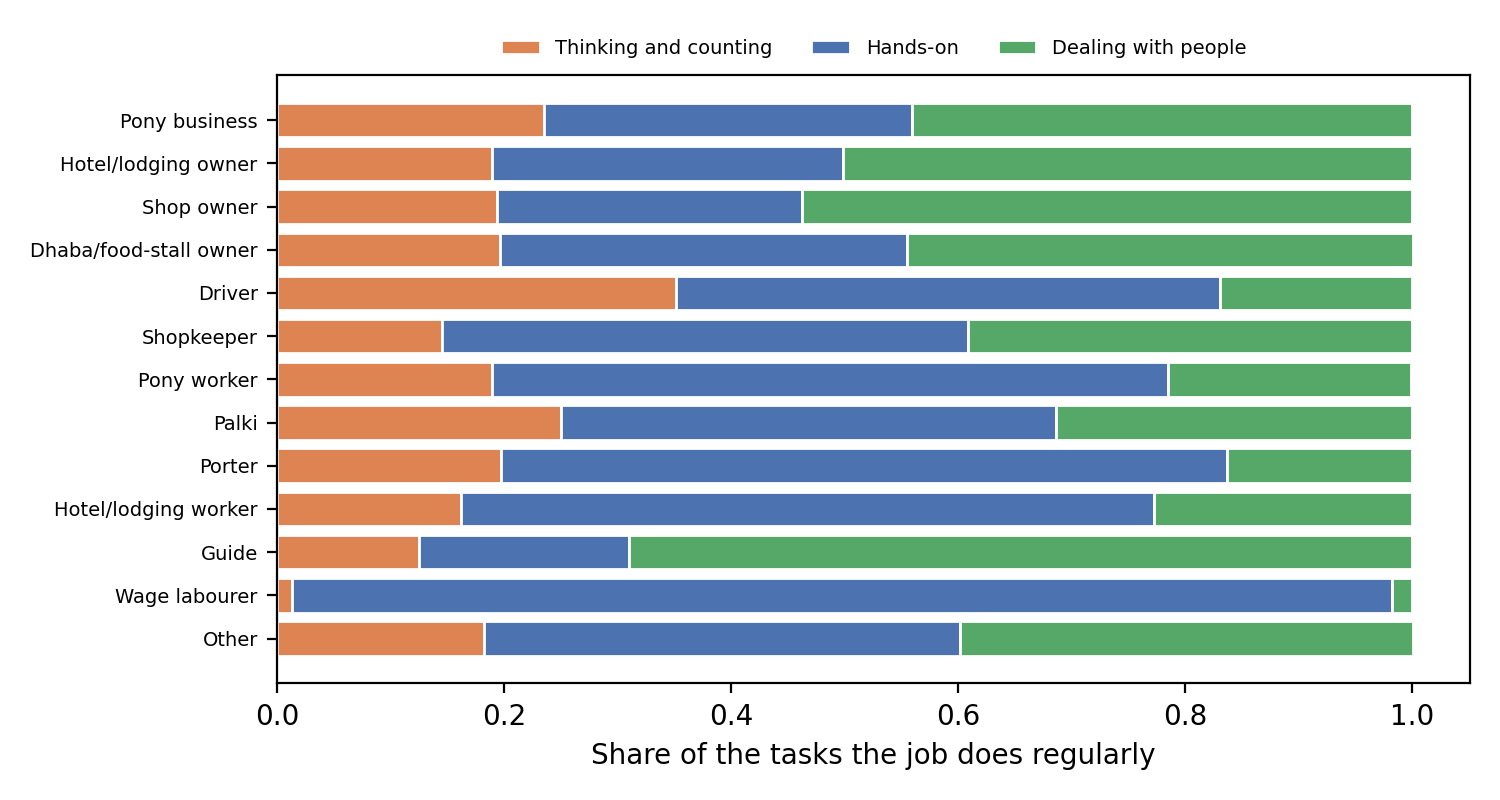
\includegraphics[width=0.85\linewidth]{../03_analysis/outputs/3_3_groups.png}\\[2pt]
{\small Share of each job's regular tasks in the three broad groups.}
\end{center}
{\small
\begin{longtable}{lrrr}
\toprule
\textbf{Job} & \textbf{Hands-on (\%)} & \textbf{With people (\%)} & \textbf{Thinking, counting (\%)} \\
\midrule
\endfirsthead
\toprule
\textbf{Job} & \textbf{Hands-on (\%)} & \textbf{With people (\%)} & \textbf{Thinking, counting (\%)} \\
\midrule
\endhead
Pony business & 32 & 44 & 24 \\
Hotel/lodging owner & 31 & 50 & 19 \\
Shop owner & 27 & 54 & 19 \\
Dhaba/food-stall owner & 36 & 45 & 20 \\
Driver & 48 & 17 & 35 \\
Shopkeeper & 46 & 39 & 14 \\
Pony worker & 60 & 21 & 19 \\
Palki & 44 & 31 & 25 \\
Porter & 64 & 16 & 20 \\
Hotel/lodging worker & 61 & 23 & 16 \\
Guide & 18 & 69 & 12 \\
Wage labourer & 97 & 2 & 1 \\
Other & 42 & 40 & 18 \\
\bottomrule
\end{longtable}
}

The finer five-way split (Part 1, section 7) gives, for all workers: hands-on varied 37 in 100,
dealing with people 32,
checking and counting repeated 15,
hands-on repeated 13 and judging varied 2.
Only one task falls in the last group, so it is too thin to use on its own. The per-job table is in the output file \texttt{3\_3\_class5\_share\_by\_job.csv}.

\section*{5. Which jobs are close to each other?}
Two jobs are close when workers in them do the same tasks. We measure this by \textbf{overlap} (a number from 0 to 1, called cosine similarity).
1 means the same tasks in the same shares; 0 means no task in common. We compute it between the average task lists of each pair of jobs.
The average overlap between two different jobs is 0.57.
{\footnotesize
\begin{longtable}{p{3.4cm}p{3.4cm}rp{3.2cm}r}
\toprule
\textbf{Job} & \textbf{Closest job} & \textbf{Overlap} & \textbf{Furthest job} & \textbf{Overlap} \\
\midrule
\endfirsthead
\toprule
\textbf{Job} & \textbf{Closest job} & \textbf{Overlap} & \textbf{Furthest job} & \textbf{Overlap} \\
\midrule
\endhead
Dhaba/food-stall owner & Hotel/lodging owner & 0.87 & Wage labourer & 0.28 \\
Driver & Palki & 0.64 & Wage labourer & 0.39 \\
Guide & Dhaba/food-stall owner & 0.66 & Wage labourer & 0.09 \\
Hotel/lodging owner & Dhaba/food-stall owner & 0.87 & Wage labourer & 0.24 \\
Hotel/lodging worker & Hotel/lodging owner & 0.70 & Wage labourer & 0.44 \\
Other & Shopkeeper & 0.90 & Palki & 0.44 \\
Palki & Porter & 0.68 & Wage labourer & 0.25 \\
Pony business & Shop owner & 0.84 & Wage labourer & 0.33 \\
Pony worker & Pony business & 0.78 & Guide & 0.37 \\
Porter & Shopkeeper & 0.76 & Guide & 0.40 \\
Shop owner & Hotel/lodging owner & 0.87 & Wage labourer & 0.26 \\
Shopkeeper & Other & 0.90 & Guide & 0.46 \\
Wage labourer & Porter & 0.65 & Guide & 0.09 \\
\bottomrule
\end{longtable}
}
\begin{center}
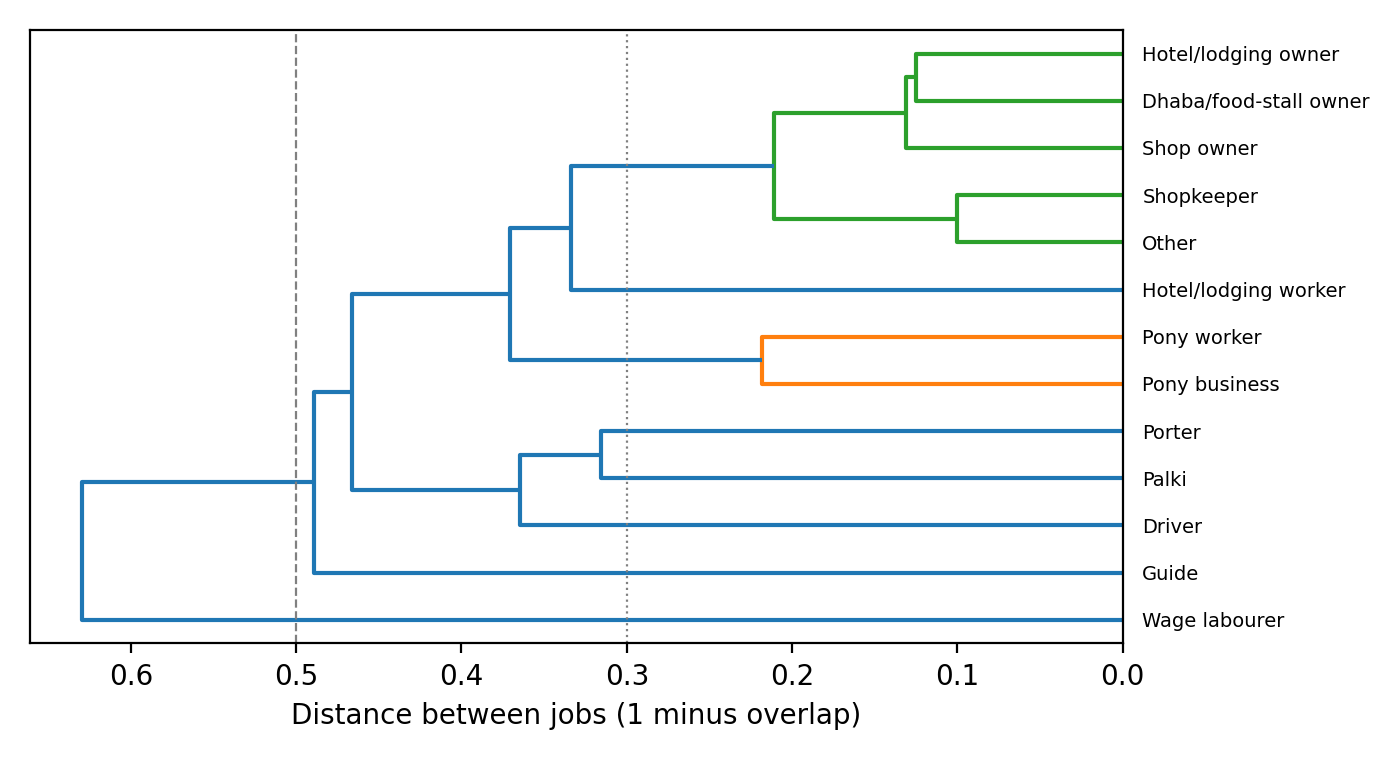
\includegraphics[width=0.8\linewidth]{../03_analysis/outputs/3_4_dendrogram.png}\\[2pt]
{\small Jobs joined step by step by task overlap. Jobs that join near the right are very alike. The dashed line is the 0.5 cut and the dotted line the 0.3 cut.}
\end{center}

We fixed one rule before looking: jobs stay together while their average overlap is at least 0.5 (a cut of 0.5).
That rule puts \textbf{2 groups}: almost all jobs together and wage labourers alone. This is not useful, because
selling, cash and carrying are so common that everyone overlaps a little. We then tried a stricter cut of 0.3 \textbf{after} seeing that result, so please treat it as exploratory. It gives 8 groups:
(Palki); (Porter); (Driver); (Pony business, Pony worker); (Dhaba/food-stall owner, Hotel/lodging owner, Other, Shop owner, Shopkeeper); (Hotel/lodging worker); (Guide); (Wage labourer).
The shop and food owners form one tight group. Ponies form a second. Porters and palki bearers are next to each other.

\textbf{Lesson for the survey.} The task list separates the trade-owner jobs from the carrying jobs well, but many jobs share a middle ground of selling, bargaining and cash.
For the ropeway question this is helpful, because the ropeway jobs also sit in that middle ground, but the group size (13 jobs, 104 workers) is too small to trust any exact cluster.

\section*{6. How different are workers inside the same job?}
Job titles are not enough to describe people. To check how much a job title explains, we asked how much of the total difference in task lists is between jobs.
\begin{itemize}[leftmargin=1.2em,itemsep=2pt]
\item Job title explains \textbf{38 in 100} of the differences (30 in 100 after allowing for the small groups).
If we shuffled job titles at random it would explain about 12 in 100. In 2000 random shuffles, none reached the real figure. So job titles matter, but most differences (about 6 in 10) are between workers in the same job.
\item Two workers in the same job have an overlap of \textbf{0.56}. Two workers in different jobs have 0.34.
\begin{center}
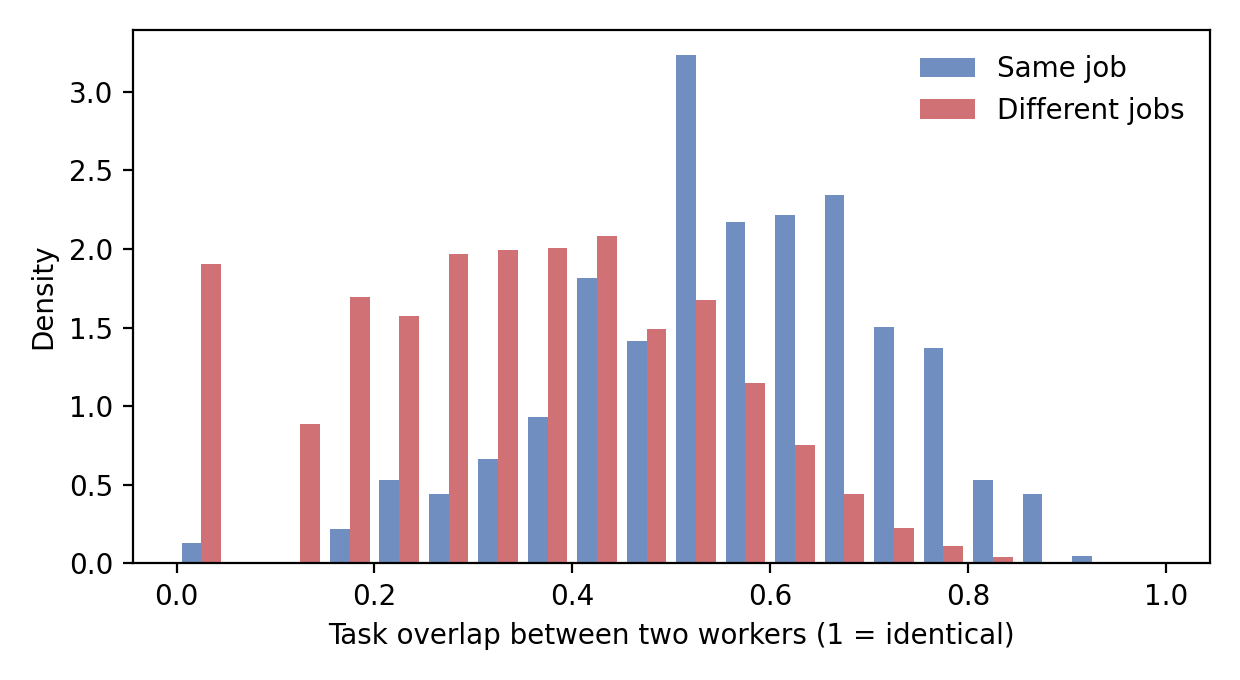
\includegraphics[width=0.65\linewidth]{../03_analysis/outputs/3_5_pairs.png}\\[2pt]
{\small Overlap between pairs of workers.}
\end{center}

\item If we hide one worker and guess the job from the tasks, the right job is the closest match for \textbf{62 in 100} workers (guessing at random would be about 1 in 13).
\end{itemize}
These figures come partly from how we built the test data (each imaginary worker has some random variation). The real survey may show more or less. What matters is that the method gives a clear reading.
The table below shows how close each worker is, on average, to the rest of their own job.
{\small
\begin{longtable}{lrrr}
\toprule
\textbf{Job} & \textbf{Workers} & \textbf{Average fit to own job} & \textbf{Lowest} \\
\midrule
\endfirsthead
\toprule
\textbf{Job} & \textbf{Workers} & \textbf{Average fit to own job} & \textbf{Lowest} \\
\midrule
\endhead
Pony business & 5 & 0.78 & 0.55 \\
Hotel/lodging owner & 7 & 0.82 & 0.73 \\
Shop owner & 11 & 0.75 & 0.58 \\
Dhaba/food-stall owner & 6 & 0.69 & 0.46 \\
Driver & 7 & 0.73 & 0.50 \\
Shopkeeper & 14 & 0.76 & 0.61 \\
Pony worker & 5 & 0.63 & 0.49 \\
Palki & 6 & 0.68 & 0.50 \\
Porter & 10 & 0.67 & 0.40 \\
Hotel/lodging worker & 15 & 0.69 & 0.53 \\
Guide & 3 & 0.46 & 0.29 \\
Wage labourer & 11 & 0.76 & 0.59 \\
Other & 4 & 0.35 & 0.25 \\
\bottomrule
\end{longtable}
}

Fit is low for ``Other'' and guides because those groups are mixed or tiny.

\section*{7. Hidden experience from other work}
Answer 2 asks about tasks done before, elsewhere. How much does it add?
\begin{itemize}[leftmargin=1.2em,itemsep=2pt]
\item 79 in 100 workers report at least one; in all, workers gave 201 such answers.
\item 72 in 100 of these are tasks that fewer than 1 in 5 of the person's own job colleagues do regularly. So most of them are \emph{new information}, which the job title would not have shown.
\item Adding them moves a worker's closest other job for 27 in 100 workers. The average gain in overlap with that job is small (0.010). The hidden tasks are common but usually small in size.
\end{itemize}
Here we compare by the person's main off-season activity. Those who work with animals or work for wages elsewhere report the most tasks done before; those with no other work report the fewest, as one would expect.
{\small
\begin{longtable}{lrrrr}
\toprule
\textbf{Off-season activity} & \textbf{Workers} & \textbf{Tasks done before (avg)} & \textbf{Any before (\%)} & \textbf{Regular tasks (avg)} \\
\midrule
\endfirsthead
\toprule
\textbf{Off-season activity} & \textbf{Workers} & \textbf{Tasks done before (avg)} & \textbf{Any before (\%)} & \textbf{Regular tasks (avg)} \\
\midrule
\endhead
Animal husbandry & 7 & 3.3 & 100 & 5.9 \\
Wage labour elsewhere & 20 & 2.4 & 90 & 8.2 \\
Agriculture & 29 & 2.3 & 90 & 7.2 \\
Migrated for work & 7 & 2.3 & 100 & 7.6 \\
Salaried job & 3 & 2.0 & 33 & 5.3 \\
Petty trade/other & 7 & 1.4 & 86 & 7.1 \\
No other work & 31 & 1.0 & 55 & 7.7 \\
\bottomrule
\end{longtable}
}
\begin{center}
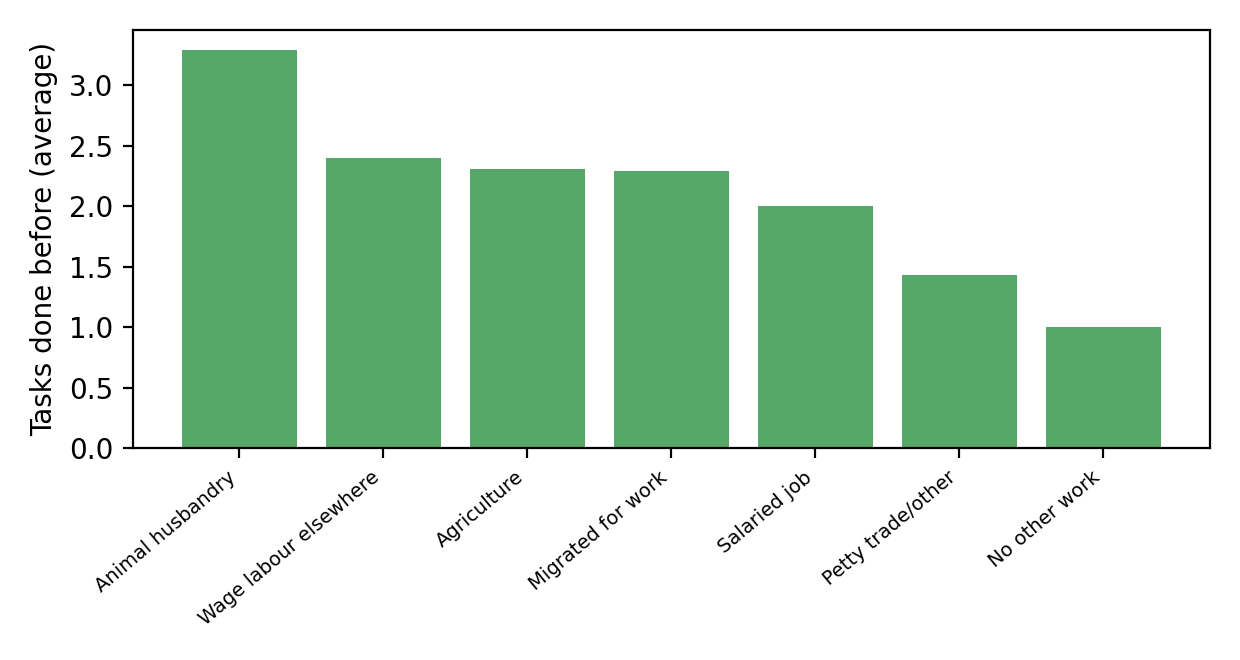
\includegraphics[width=0.65\linewidth]{../03_analysis/outputs/3_6_hidden.png}\\[2pt]
{\small Average number of tasks done before elsewhere, by off-season activity.}
\end{center}

\textbf{Note.} This pattern is built into the test data on purpose (Part 2, step 3). Real data may not show it. If the real answer 2 does not vary with off-season work,
either the question is not working or the assumption is wrong. That is a useful test in the field.

\section*{8. What we learn for the survey}
\begin{enumerate}[leftmargin=1.4em,itemsep=2pt]
\item The 27-task list separates jobs reasonably well. Keep it.
\item Guides and ``Other'' need more workers, or must be pooled. With 3 or 4 workers nothing can be said.
\item Answer 2 gives new information for most workers. Keep it, but check in the pilot that people understand ``done before''.
\item Some tasks are rare (engine, electrical work, teaching, carrying a passenger). A count alone would drop them, but we keep them because ropeway jobs may need them.
\item The job-by-job overlap will change once real data are in. All code here can be run again unchanged.
\end{enumerate}

\section*{9. Files}
\begin{itemize}[leftmargin=1.2em,itemsep=1pt]
\item \texttt{03\_analysis/general\_analysis.py}: the code. \texttt{03\_analysis/results\_general.json}: all numbers.
\item \texttt{03\_analysis/outputs/}: tables (\texttt{3\_1} to \texttt{3\_6}, \texttt{.csv}) and pictures (\texttt{.png}).
\end{itemize}
\end{document}
